% $Id: INF_Poster_example.tex 7714 2011-08-31 17:34:46Z tkren $
%
% TU Wien - Faculty of Informatics
% poster template
%
% This template is using the beamer document class and beamerposter package, see
% <http://www.ctan.org/tex-archive/macros/latex/contrib/beamer/>
% <http://www.ctan.org/tex-archive/macros/latex/contrib/beamerposter/>
% <http://www-i6.informatik.rwth-aachen.de/~dreuw/latexbeamerposter.php>
%
% For questions and comments send an email to
% Thomas Krennwallner <tkren@kr.tuwien.ac.at>
%

\documentclass[final,hyperref={pdfpagelabels=true}]{beamer}

\usepackage{TUINFPST}

\usepackage{lipsum}

%\title[Computational Intelligence]{Interactive Computer Generated Architecture}
% if you have a long title looking squeezed on the poster, just force
% some distance:
\title[Software Engineering \& Internet Computing]{A Big Data Analytics Framework for Evaluating Automated Elastic Scalability of the SMACK-Stack}
\author[benedikt.wedenik@alumni.tuwien.ac.at]{Benedikt Wedenik}
\institute[]{%
  Technische Universit{\"a}t Wien\\[0.25\baselineskip]
  Institut f{\"u}r Informationssysteme\\[0.25\baselineskip]
  Arbeitsbereich: Distributed Systems Group\\[0.25\baselineskip]
  Betreuer: Univ.Prof. Mag.rer.soc.oec. Dr.rer.soc.oec. Schahram Dustdar
}
\titlegraphic{
\includegraphics[height=52mm]{logo_184-1}}
\date[\today]{\today}
\subject{epilog}
\keywords{Big Data / Cloud Computing / SMACK-Stack / Scalability / Data Analytics}

%%%%%%%%%%%%%%%%%%%%%%%%%%%%%%%%%%%%%%%%%%%%%%%%%%%%%%%%%%%%%%%%%%%%%%%%%%%%%%%%%%%%%%

% Display a grid to help align images
%\beamertemplategridbackground[12.7mm]

% play around with the background colors
% \setbeamercolor{background canvas}{bg=yellow}

% use a background picture
% \usebackgroundtemplate{%
%   \includegraphics[width=\paperwidth]{logo_KBS_2_CMYK}
% }

% play around with block colors
\setbeamercolor{block body}{fg=black,bg=white}
\setbeamercolor{block title}{fg=TuWienBlue,bg=white}

\setbeamertemplate{block begin}{
  \begin{beamercolorbox}{block title}%
    
\begin{tikzpicture}%
      \node[draw,rectangle,line width=3pt,rounded corners=0pt,inner sep=0pt]{%
        \begin{minipage}[c][2cm]{\linewidth}
          \centering\textbf{\insertblocktitle}
        \end{minipage}
      };
    \end{tikzpicture}%
  \end{beamercolorbox}
  \vspace*{1cm}
  \begin{small}
  \begin{beamercolorbox}{block body}%
}

\setbeamertemplate{block end}{
  \end{beamercolorbox}
  \end{small}
  \vspace{2cm}
}

% setup postit
\setbeamercolor{postit}{fg=black,bg=yellow}
\newenvironment{postit}
{\begin{beamercolorbox}[sep=1em,wd=7cm]{postit}}
{\end{beamercolorbox}}


% for crop marks, uncomment the following line
%\usepackage[cross,width=88truecm,height=123truecm,center]{crop}

%%%%%%%%%%%%%%%%%%%%%%%%%%%%%%%%%%%%%%%%%%%%%%%%%%%%%%%%%%%%%%%%%%%%%%%%%%%%%%%%%%%%%%

\begin{document}

% We have a single poster frame.
\begin{frame}
  \begin{columns}[t]
    % ---------------------------------------------------------%
    % Set up a column
    \begin{column}{.48\textwidth}
      \begin{block}{Motivation \& Research Challenges}
	In the last years the demand for information availability and shorter response times has been increasing.
	Today's business requirements are changing: Waiting hours or even days for the result of a query is not acceptable anymore in many sectors.
	The response needs to be immediate, or the query is discarded \cite{estrada2016big}.
	This is why "Fast Data", as an approach to solve those problems, increases its popularity, as being "big data, but fast" \cite{mishne2013fast}.\\
	\hfill \\

	\begin{itemize}
	\item \textbf{Deploying large scale applications} \\
		Requires multiple instances of different technologies to be deployed in a defined sequence to fulfill subsequent dependencies, often including manual steps.
	\item \textbf{Initial setup} \\
		The decision of how to configure the instances of an application is a non-trivial task, as there are almost infinite combination possibilities and the impact can be drastic.
	\item \textbf{Monitoring} \\
		Considering just RAM, CPU and disk usage is in most cases insufficient, as a deeper understanding of the used frameworks is required, which introduces a new layer of complexity.
	\item \textbf{Scaling when needed} \\
		Understanding what’s going on in a cluster and reacting accordingly is crucial for the success of any large scale application.
	\end{itemize}
      \end{block}

      \begin{block}{Contributions}
	To solve the problems mentioned above, the framework illustrated in Figure~\ref{fig:architecture} has been developed in the course of this thesis, whereas the single components can be described as follows:\\
	\hfill \\

	\begin{itemize}
  	  \item \textbf{Automated Scaling Tool for SMACK}\\
          The scaling tool evaluates the collected metrics from the REST service and scales the individual parts of the SMACK stack up or down.
   	 \item \textbf{REST Service Collecting Monitoring Information}\\
          This is the service which collects all the extracted metrics and compiles them into a useful format.
          In addition, there is the possibility to generate plots at runtime.
  	  \item \textbf{JMX Extraction Tool}\\
          This tool is designed to automatically extract interesting metrics from SMACK components via JMX and sending them to a central service, in this case the REST monitoring service.
   	 \item \textbf{Framework to Easily Launch SMACK in AWS}\\
          With the help of this framework it takes just a few command line calls to launch and deploy the whole SMACK stack in the cloud.
   	 \item \textbf{Deployment Blueprints}\\
          Those reference architecture and configuration recommendations help to launch the SMACK stack and getting most out of the available resource.
	\end{itemize}
		\hfill \\ \hfill \\

	\begin{figure}[!htbp]
  		\centering
 		 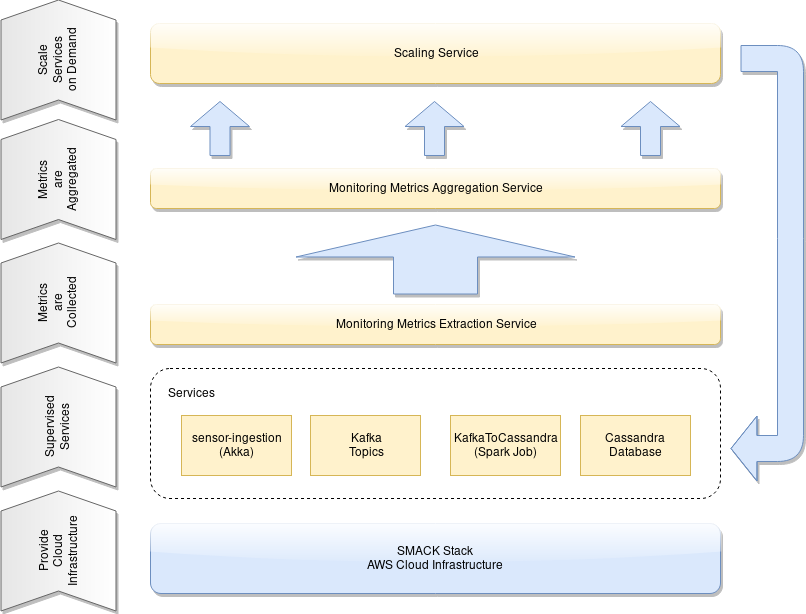
\includegraphics[keepaspectratio=true,scale=1.3]{figures/architecture}
  		  \caption{Framework Target Architecture}
  		  \label{fig:architecture}
	\end{figure}
      \end{block}


    \end{column}
    % ---------------------------------------------------------%
    % end the column

    % ---------------------------------------------------------%
    % Set up a column
    \begin{column}{.48\textwidth}
      \begin{block}{Background}
		The SMACK-Stack consists of five technologies combined to a lightning fast data pipeline for today's needs of big data applications, as shown in Figure~\ref{fig:smack_stack}.\\
		\hfill \\

		\begin{figure}[!htbp]
  			\centering
  			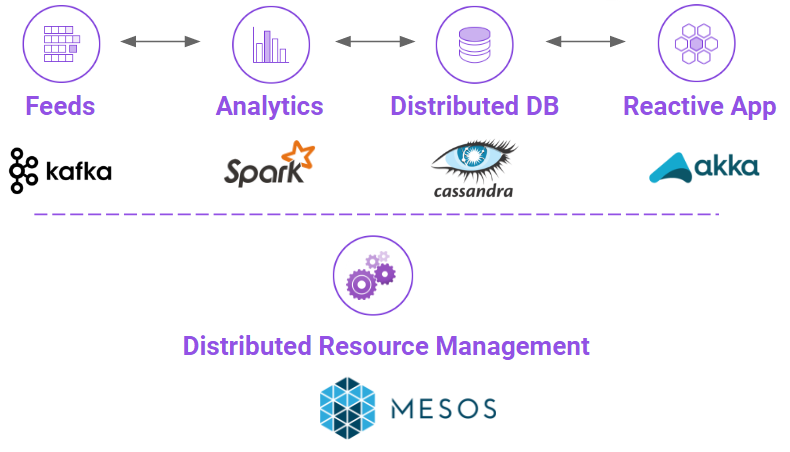
\includegraphics[keepaspectratio=true,scale=1.1]{figures/smack_stack}
    			\caption{SMACK Stack Illustration, mesosphere.com}
  			\label{fig:smack_stack}
		\end{figure}

	\hfill \\

		\begin{itemize}
 		   \item Apache \textbf{S}park is the engine of the pipeline, providing batch-, as well as stream-processing power for large-scale data processing.
   		 \item \textbf{M}esos is a datacenter operating system with the aim to reduce complexity and ease the deployment and maintenance of large-scale distributed applications.
   		 \item Apache \textbf{A}kka can be seen as the model, providing the possibility to build powerful reactive distributed message-driven applications.
   		 \item Apache \textbf{C}assandra is a highly distributed database which is a hybrid between a column-oriented and a key-value DBMS, which is implemented avoiding a single point of failure.
   		 \item Apache \textbf{K}afka serves as publish-subscribe message broker, which is usually the ingestion point of the pipeline.
		\end{itemize}

      \end{block}

      \begin{block}{Results \& Conclusion}
	As part of the contribution, two real world applications have been developed in order to provide a valid base for the evaluation of the framework.
	The \textit{IoT Data Storage Application} is mainly I/O bound and represents applications which require high throughput.
	In case of the \textit{Acceleration Prediction Application}, a prediction based on IoT data is performed, which is heavily computational intense.\\
	\hfill \\

	To evaluate the actual impact of the framework, empirical experiments have been conducted.
	The setup comprises one run without the framework - i.e. unsupervised, which serves as a baseline, and a supervised one, in which the framework automatically scales the respective services.
	When analyzing the measured results, both applications benefit from the scaling service, where the following improvements can be highlighted:\\
	\hfill \\

	\begin{itemize}
		\item An \textbf{increase from 272 to 472 MBit/s} was measured when running the \textit{IoT Data Storage Application}, as well as other \textbf{metrics like the time-in-mailbox of a message were improved}.
		\item The \textit{Acceleration Prediction Application} benefited in form of \textbf{shorter message processing times} and an overall \textbf{faster task completion}.
	\end{itemize}
      \end{block}

\hfill \\ \hfill \\ \hfill \\  \hfill \\  \hfill \\
      \begin{block}{References}
		\begin{footnotesize}
			\bibliographystyle{abbrv}
			\bibliography{cites}
		\end{footnotesize}
      \end{block}

    \end{column}
    % ---------------------------------------------------------%
    % end the column

  \end{columns}


%  \begin{tikzpicture}[remember picture,overlay]
%    \node[inner sep=0pt,xshift=-30cm,yshift=53cm] at (current page.east) {%
%      \begin{postit}%
%        Post-It time!%
%      \end{postit}%
%    };
%  \end{tikzpicture}

\end{frame}

\end{document}

%%% Local Variables:
%%% TeX-PDF-mode: t
%%% TeX-debug-bad-boxes: t
%%% TeX-master: t
%%% TeX-parse-self: t
%%% TeX-auto-save: t
%%% reftex-plug-into-AUCTeX: t
%%% End:
